%%%%%%%%%%%%%%%%%%%%%%%%%%%%%%%%%%%%%%%%%%%%%%%%%%%%%%%%%%%%%%%%%%%%%%%%%%%%%%%%
%% 
\cleardoubleoddpage%  Make sure to start each chapter on a new odd page
\chapter{Methodology}
\label{sec:methodology}

This chapter presents the experimental methodology used to evaluate \ac{xLSTM} architectures within the \ac{BIOT} framework for \ac{EEG} event classification. The focus is on the conceptual framework, scientific rationale, and research design that guides the experimental evaluation.

\section{Experimental Framework}
\label{sec:experimental_framework}

The experimental framework builds upon the existing \ac{BIOT} architecture by integrating \ac{xLSTM} components as alternatives to the traditional Transformer encoder layers. This integration aims to evaluate whether the enhanced memory mechanisms of \ac{xLSTM} can improve the model's ability to capture long-range dependencies in \ac{EEG} sequences while maintaining computational efficiency.

\subsection{Research Questions and Objectives}
\label{sec:research_questions}

The primary research questions guiding this experimental evaluation are:

\begin{enumerate}
    \item \textbf{Performance Comparison}: How do \ac{xLSTM} variants (\ac{sLSTM}, \ac{mLSTM}, and their combination) compare to the original \ac{BIOT} architecture for \ac{EEG} event classification?
    
    \item \textbf{Temporal Context}: What is the optimal temporal window size for capturing relevant context around clinical \ac{EEG} events?
    
    \item \textbf{Architectural Components}: What are the individual contributions of \ac{sLSTM} and \ac{mLSTM} components to overall classification performance?
    
    \item \textbf{Robustness}: How consistent is model performance across different random initializations and class distributions?
\end{enumerate}

These questions are addressed through systematic experimentation with controlled parameter variations, enabling clear attribution of performance differences to specific architectural choices.

\subsection{Integration Strategy}
\label{sec:integration_strategy}

The integration of \ac{xLSTM} into the \ac{BIOT} framework preserves the core tokenization and preprocessing mechanisms while replacing the sequence modeling components. This modular approach enables fair comparison by isolating the impact of different sequence modeling architectures.

Key integration principles include:
\begin{itemize}
    \item \textbf{Tokenization Preservation}: The biosignal tokenization module remains unchanged, ensuring all models process identical input representations
    \item \textbf{Dimensional Consistency}: All encoder variants maintain the same embedding dimensions and token lengths
    \item \textbf{Architectural Modularity}: The encoder component can be replaced without modifying preprocessing or classification layers
    \item \textbf{Compatibility}: Both \ac{sLSTM} and \ac{mLSTM} variants operate on the same tokenized input format
\end{itemize}

This integration strategy maintains the advantages of \ac{BIOT}'s flexible tokenization while enabling systematic evaluation of different temporal sequence modeling approaches.

\subsection{Model Variants}
\label{sec:model_variants}

Four distinct model variants are evaluated to systematically assess the impact of different \ac{xLSTM} components:

\textbf{BIOT Baseline:} The original \ac{BIOT} architecture with Linear Attention Transformer serves as the baseline for comparison. This configuration provides the reference performance against which \ac{xLSTM} enhancements are measured.

\textbf{sLSTM:} This configuration replaces the Transformer encoder with \ac{sLSTM} blocks featuring scalar memory mechanisms and exponential gating. The \ac{sLSTM} variant emphasizes sequential processing with memory mixing, potentially improving the model's ability to track evolving patterns in \ac{EEG} sequences.

\textbf{mLSTM:} This configuration employs \ac{mLSTM} blocks with matrix memory structures, enabling enhanced storage capacity through key-value associations. The \ac{mLSTM} variant is fully parallelizable, offering computational efficiency while maintaining rich representational capabilities.

\textbf{sLSTM + mLSTM:} The combined configuration integrates both memory mechanisms in a unified architecture, leveraging the complementary strengths of scalar and matrix memory. This variant represents the most complex model with the highest representational capacity.

Each variant is evaluated under identical training conditions and data processing pipelines, enabling direct performance attribution to the architectural differences in sequence modeling.


\section{Dataset: Temple University Hospital EEG Event Corpus}
\label{sec:dataset}

\subsection{Background and Motivation}
\label{sec:dataset_background}

Clinical \ac{EEG} data represents a valuable yet still underexploited resource for machine learning research. Although large volumes of \ac{EEG} are recorded in hospitals worldwide, comparatively few datasets are available in forms suitable for algorithm development \cite{obeid2016temple}. This scarcity poses challenges, as modern deep learning approaches typically benefit from large and diverse datasets to achieve robust performance.

The \ac{TUH} \ac{EEG} Corpus was established to address this limitation by providing a large-scale clinical \ac{EEG} database to the research community. It comprises 16,986 sessions from 10,874 subjects collected between 2002 and the present, corresponding to approximately 29.1 years of cumulative recording time \cite{obeid2016temple}. The corpus contains clinical-grade \ac{EEG} recorded across multiple hospital environments, including intensive care units, epilepsy monitoring units, emergency departments, and outpatient services.

The \ac{TUEV} subset was created specifically to support research on \ac{EEG} event classification and includes sessions annotated for clinically meaningful events such as epileptiform discharges, in addition to artifacts and eye movements \cite{harati2015improved}. This makes the dataset particularly suitable for developing and evaluating automated event detection and classification systems, which may support neurologists in analyzing long-term \ac{EEG} recordings.

\subsection{Dataset Structure and Organization}
\label{sec:dataset_structure}

The \ac{TUEV} dataset is organized into distinct training and evaluation partitions, consisting of 359 and 159 \ac{EEG} files respectively. This separation ensures that model evaluation is conducted on sessions that are independent from those used during training.

Signal data is stored in the \ac{EDF}, an open-source format that encodes multi-channel time-series data using 16-bit integers. Each \ac{EDF} file contains both the raw \ac{EEG} signals and associated metadata in an ASCII header describing channel labels, sampling rates, and recording parameters. The recordings represent pruned clinical \ac{EEG} segments in which sections marked as uninformative by technicians were removed, yielding focused intervals that predominantly contain clinically reviewed activity.

The file organization follows a hierarchical structure that preserves relationships between recordings. For the evaluation set, files are organized by session index (e.g., \texttt{eval/032/bckg\_032\_a\_.edf}), where multiple files may represent segments from the same recording session. For the training set, files are indexed by patient identifier (e.g., \texttt{train/00002275/00002275\_00000001.edf}), allowing sessions from the same patient to be identified and grouped appropriately during data partitioning.

\subsection{Event Classes and Clinical Significance}
\label{sec:event_classes}

The \ac{TUEV} dataset annotates six distinct classes of events, three representing clinically significant neural patterns and three representing various forms of background activity or noise:

\textbf{Clinical Event Classes:}
\begin{itemize}
    \item \textbf{\ac{SPSW}:} Epileptiform transients characterized by sharp waveforms typically observed in patients with epilepsy. These events represent abnormal synchronized neural activity and are critical markers for seizure disorders.
    
    \item \textbf{\ac{GPED}:} Periodic discharges that manifest as repetitive patterns distributed across multiple brain regions. These can appear as periodic short-interval diffuse discharges, periodic long-interval diffuse discharges, or suppression-burst patterns, and may indicate severe brain dysfunction.
    
    \item \textbf{\ac{PLED}:} Lateralized periodic discharges that appear repetitively over one hemisphere. These quasi-periodic spike or sharp wave patterns are indicative of focal brain abnormalities and often manifest in patients with acute neurological conditions.
\end{itemize}

\textbf{Background and Noise Classes:}
\begin{itemize}
    \item \textbf{\ac{EYEM}:} Ocular artifacts generated by eye movements. These events can mimic spike patterns in frontal electrodes and must be distinguished from true epileptiform activity during clinical interpretation.
    
    \item \textbf{\ac{ARTF}:} Non-cerebral electrical activity originating from equipment, patient movement, muscle activity, or environmental interference. Artifact detection is essential for maintaining data quality and preventing false positives in clinical analysis.
    
    \item \textbf{\ac{BCKG}:} Background \ac{EEG} activity that does not belong to any of the other five classes. This catch-all category represents normal or non-specific brain activity.
\end{itemize}

Event annotations are provided in two complementary formats. The \texttt{.rec} files contain comma-separated records specifying: channel number (0-21), start time in seconds, end time in seconds, and event class (1-6). The \texttt{.lab} files provide the same information with timestamps in units of 10 microseconds and four-letter class codes (spsw, gped, pled, eyem, artf, bckg). This dual format supports both machine parsing and human interpretation.

\subsection{Class Distribution and Imbalance}
\label{sec:class_distribution}

The distribution of events varies significantly across the training and evaluation sets, reflecting the natural distribution of events in clinical practice. In the training set, background activity is present in the largest number of files (211 files), whereas clinically relevant events such as \ac{SPSW} appear in comparatively fewer files (27 files). These numbers refer to files containing at least one instance of the corresponding event type rather than individual event counts. The evaluation set shows similar patterns with artifacts in 46 files and \ac{SPSW} in only 9 files.

This class imbalance presents a significant challenge for machine learning algorithms, which tend to bias predictions toward majority classes. The imbalance necessitates:
\begin{itemize}
    \item Evaluation metrics that account for class imbalance (balanced accuracy, Cohen's Kappa)
    \item Careful interpretation of overall accuracy metrics
    \item Potential class-specific performance analysis
    \item Consideration of clinical cost asymmetries (false negatives vs. false positives)
\end{itemize}

The imbalanced distribution reflects real-world clinical scenarios where pathological events are less frequent than normal background activity, making this dataset particularly valuable for developing clinically applicable algorithms.

\subsection{Electrode Configuration and Channel System}
\label{sec:electrode_configuration}

Understanding the electrode configuration and channel labeling system is crucial for correctly interpreting \ac{EEG} data from the \ac{TUEV} dataset. The recordings follow standardized electrode placement protocols that enable consistent spatial localization of neural activity.

\textbf{International 10-20 Electrode System:} The \ac{TUEV} recordings use the International 10-20 system, the most widely adopted standard for \ac{EEG} electrode placement (see Figure~\ref{fig:10_20_system}). This system positions 21 electrodes on the scalp with spacing determined by 10\% or 20\% of the total distance from nasion (front of skull) to inion (back of skull) \cite{ferrell2022electrode}. Electrode names follow a systematic convention where letters indicate brain region (Fp=prefrontal, F=frontal, C=central, T=temporal, P=parietal, O=occipital, A=auricular) and numbers indicate laterality (odd=left hemisphere, even=right hemisphere, Z=midline).

\begin{figure}[htbp]
    \centering
    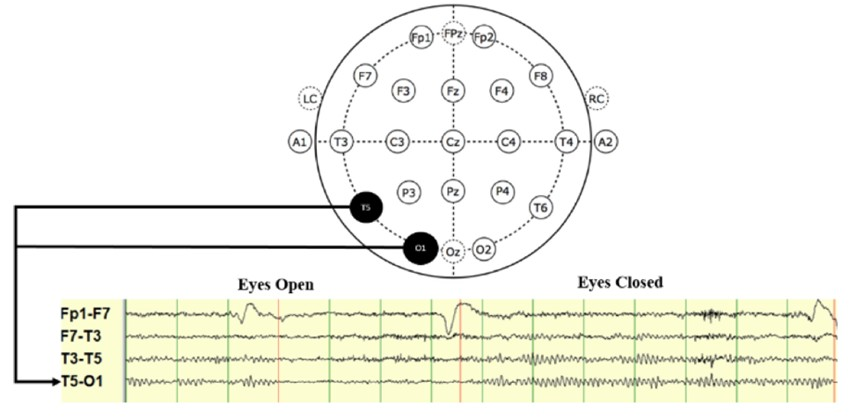
\includegraphics[width=0.8\textwidth]{images/eeg_10_20_system.jpg}
    \caption{International 10-20 electrode system showing the standardized placement of electrodes on the scalp (adapted from~\cite{ferrell2022electrode}). The system uses anatomical landmarks (nasion, inion, and preauricular points) to ensure consistent electrode positioning across subjects.}
    \label{fig:10_20_system}
\end{figure}

\textbf{Unipolar Recording Montages:} Raw \ac{EEG} signals are recorded as differential voltages between individual electrodes and a reference point, a process known as unipolar recording. The \ac{TUEV} dataset contains recordings using two primary unipolar montages: \ac{AR} montage, which uses the average of multiple electrodes as the reference, and \ac{LE} montage, which links the left and right ear electrodes (A1 and A2) to provide a stable reference point \cite{ferrell2022electrode}.

\textbf{Channel Labels and Variability:} Each channel in an \ac{EDF} file is identified by a label such as ``EEG FP1-REF'' or ``EEG C3-REF'', where the electrode name is followed by the reference type \cite{ferrell2022electrode}. An important characteristic of clinical data is that channels do not appear in a guaranteed order within files. Different recording sessions may store the same electrode in different positions, requiring software to access channels by label rather than assuming fixed positions. The complete \ac{TUH} corpus contains over 40 different channel configurations, reflecting the reality of data collected across different hospital units, equipment generations, and clinical protocols.


\section{Data Preprocessing Pipeline}
\label{sec:preprocessing}

The preprocessing pipeline transforms raw \ac{EEG} recordings into a format suitable for neural network training while preserving the temporal and spatial characteristics essential for event classification. This section describes the conceptual approach and rationale for each preprocessing stage.

\subsection{Bipolar Montage Conversion}
\label{sec:bipolar_montage}

While the raw \ac{EEG} data is recorded using unipolar montages with a common reference, neurologists typically analyze \ac{EEG} signals using bipolar montages for clinical interpretation. A bipolar montage represents the voltage difference between pairs of adjacent electrodes, which provides several advantages:

\begin{itemize}
    \item \textbf{Local Feature Enhancement}: Bipolar derivations accentuate local neural activity by measuring potential differences between nearby electrodes
    \item \textbf{Common-Mode Artifact Rejection}: Artifacts affecting large scalp regions simultaneously are reduced through differential measurement
    \item \textbf{Clinical Consistency}: Bipolar montages closely align with representations commonly used by neurologists for visual analysis, facilitating clinical validation
    \item \textbf{Spatial Localization}: Local voltage gradients can improve spatial discrimination of event origins compared to purely reference-based recordings
\end{itemize}

The preprocessing pipeline converts unipolar recordings to a standard \ac{TCP} bipolar montage, also known as the double-banana montage due to its characteristic visualization pattern (see Figure~\ref{fig:tcp_montage}). The \ac{TCP} montage creates 22 channels by computing differences between adjacent electrodes along electrode chains.

\begin{figure}[htbp]
    \centering
    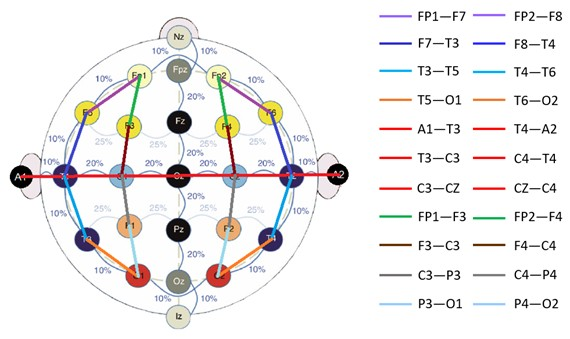
\includegraphics[width=0.7\textwidth]{images/tcp_montage.jpg}
    \caption{Temporal Central Parasagittal (TCP) montage showing the electrode chains used for bipolar derivations (adapted from~\cite{ferrell2022electrode}). The longitudinal chains traverse from front to back through temporal regions, while parasagittal chains pass near the midline. This montage is commonly referred to as the ``double-banana'' configuration.}
    \label{fig:tcp_montage}
\end{figure}

\textbf{Longitudinal Chains} traverse from front to back across the temporal regions:
\begin{itemize}
    \item Left temporal: FP1-F7, F7-T3, T3-T5, T5-O1
    \item Right temporal: FP2-F8, F8-T4, T4-T6, T6-O2
\end{itemize}

\textbf{Parasagittal Chains} traverse from front to back near the midline:
\begin{itemize}
    \item Left parasagittal: FP1-F3, F3-C3, C3-P3, P3-O1
    \item Right parasagittal: FP2-F4, F4-C4, C4-P4, P4-O2
\end{itemize}

\textbf{Central Chain} crosses laterally across the midline:
\begin{itemize}
    \item Transverse: A1-T3, T3-C3, C3-CZ, CZ-C4, C4-T4, T4-A2
\end{itemize}

For this work, 16 of these 22 channels are utilized, omitting the transverse chain components that include auricular electrodes. This selection provides comprehensive spatial coverage while maintaining consistency across recordings.

\subsection{Signal Resampling}
\label{sec:signal_resampling}

The raw \ac{EEG} signals are recorded at varying sampling rates across different recording sessions. Signal resampling standardizes the temporal resolution across all recordings, enabling consistent temporal analysis. The resampling from the original 250 Hz to 200 Hz serves multiple purposes:

\begin{itemize}
    \item \textbf{Standardization}: Ensures all signals have identical temporal resolution
    \item \textbf{Nyquist Criterion}: Maintains sufficient sampling for frequency content up to 100 Hz, covering the clinical frequency range of interest (0.5-50 Hz)
    \item \textbf{Computational Efficiency}: Reduces the number of time points while preserving clinically relevant information
\end{itemize}

The resampling operation employs anti-aliasing filters to prevent spectral distortion and artifacts, ensuring the integrity of frequency-domain features used in subsequent processing stages.

\subsection{Signal Normalization}
\label{sec:signal_normalization}

Each channel undergoes normalization by scaling to the 95th percentile of absolute signal amplitudes. This approach divides each channel's values by its 95th percentile, bringing all channels to a comparable amplitude range while maintaining robustness against extreme values.

The percentile-based normalization offers several advantages for clinical \ac{EEG} data:

\begin{itemize}
    \item \textbf{Robust to Outliers}: Large-amplitude artifacts or pathological events do not dominate the scaling factor, unlike mean-based or maximum-based approaches
    \item \textbf{Channel Consistency}: Different channels and recording sessions are normalized to comparable scales, facilitating cross-channel learning
    \item \textbf{Preserves Temporal Patterns}: The relative amplitude relationships within each channel remain intact, maintaining clinically relevant signal dynamics
\end{itemize}

This normalization strategy provides stable scaling across diverse recording conditions while preserving the amplitude patterns essential for distinguishing different event types.

\subsection{Event Window Extraction}
\label{sec:event_windows}

The event extraction process creates fixed-length windows centered around annotated events, enabling consistent input dimensions for neural network training while capturing relevant temporal context. This windowing approach addresses several key challenges:

\textbf{Temporal Context Capture:} Clinical interpretation of \ac{EEG} events requires context around the annotated event. Activity preceding an event may represent buildup patterns, while post-event activity may indicate resolution or evolution. The configurable window approach enables systematic investigation of optimal context length.

\textbf{Fixed-Size Input Requirement:} Neural networks typically require fixed-size inputs for efficient batch processing. The windowing approach transforms variable-length annotated events into uniform representations suitable for modern deep learning frameworks.

\textbf{Multi-channel Spatial Context:} Events are extracted across all 16 bipolar channels, not just the annotated channel. This provides spatial context and enables the model to learn patterns that may involve multiple brain regions, improving classification robustness.

The window extraction strategy employs configurable parameters (\texttt{secondsBefore} and \texttt{secondsAfter}) that define the temporal extent around each event. This parameterized design enables systematic exploration of different temporal contexts through experimental variation, which is crucial for identifying the optimal window size for classification performance.


\section{Experimental Design}
\label{sec:experimental_design}

\subsection{Training Strategy}
\label{sec:training_strategy}

The training approach employs supervised learning with careful attention to data partitioning and validation strategy. The experimental design emphasizes reproducibility, robust evaluation, and systematic comparison across model variants.

\textbf{Data Partitioning Philosophy:} The dataset is partitioned into three distinct sets with clear purposes:
\begin{itemize}
    \item \textbf{Training set:} Used for model parameter optimization through gradient descent
    \item \textbf{Validation set:} Used for hyperparameter tuning, model selection, and early stopping decisions
    \item \textbf{Test set:} Reserved for final unbiased performance assessment
\end{itemize}

Critically, the validation split is performed at the subject level rather than the sample level. This ensures that all samples from the same subject remain within the same partition, preventing data leakage that would artificially inflate performance estimates. Subject-level splitting provides more realistic assessment of model generalization to new patients, which is the ultimate goal in clinical applications.

\textbf{Reproducibility Requirements:} To enable reproducible research and facilitate comparison with future work:
\begin{itemize}
    \item Fixed random seeds are applied consistently across all random number generators
    \item Data loading order is standardized through sorted file lists
    \item Subject-level splitting uses fixed random states for consistency
\end{itemize}

These measures ensure that reported results can be reliably reproduced and that performance differences reflect true architectural improvements rather than random initialization effects.

\subsection{Evaluation Methodology}
\label{sec:evaluation_methodology}

The evaluation methodology employs multiple metrics to provide comprehensive assessment of model performance across different aspects of the classification task. The metric selection addresses the specific challenges of clinical \ac{EEG} event classification.

\subsection{Evaluation Metrics}
\label{sec:evaluation_metrics}

\textbf{Primary Metric - Balanced Accuracy:} Balanced accuracy serves as the primary evaluation metric due to the significant class imbalance in the \ac{TUEV} dataset. Unlike standard accuracy, which can be misleadingly high when a model simply predicts the majority class, balanced accuracy computes the average recall across all classes:

\begin{equation}
\text{BACC} = \frac{1}{K} \sum_{i=1}^{K} \frac{TP_i}{TP_i + FN_i}
\end{equation}

where $K$ is the number of classes, $TP_i$ denotes true positives for class $i$, and $FN_i$ denotes false negatives. For the 6-class \ac{TUEV} problem, each class contributes equally (16.67\%) to the final score regardless of class frequency. This ensures that rare but clinically important events like \ac{SPSW} receive equal weight to common events like artifacts.

\textbf{Secondary Metrics:} Additional metrics provide complementary perspectives on model performance:

\textbf{Weighted F1-Score} balances precision and recall while accounting for class frequency:
\begin{equation}
F1_{weighted} = \sum_{i=1}^{K} w_i \cdot \frac{2 \cdot Precision_i \cdot Recall_i}{Precision_i + Recall_i}
\end{equation}
where $w_i = \frac{n_i}{n_{total}}$ is the proportion of samples in class $i$. This metric is computed per-class then averaged with support-based weights.

\textbf{Cohen's Kappa} accounts for chance agreement, providing robust assessment beyond simple accuracy:
\begin{equation}
\kappa = \frac{p_o - p_e}{1 - p_e}
\end{equation}
where $p_o$ is observed agreement (accuracy) and $p_e$ is expected agreement under independence:
\begin{equation}
p_e = \sum_{i=1}^{K} \frac{(TP_i + FP_i)(TP_i + FN_i)}{n_{total}^2}
\end{equation}

\textbf{AUC-PR Macro} evaluates performance using precision-recall curves, which are particularly informative for imbalanced datasets because they emphasize performance on the positive (rare) class. For each class, a one-vs-rest precision-recall curve is computed, its area under the curve is obtained, and the results are averaged across classes:
\begin{equation}
\text{AUC-PR}_{macro} = \frac{1}{K} \sum_{i=1}^{K} \int Precision_i(Recall_i) \, dRecall_i
\end{equation}

Macro-averaging ensures that each class contributes equally to the final score, regardless of its frequency.

\textbf{Overall Accuracy} provides intuitive performance understanding:
\begin{equation}
\text{Accuracy} = \frac{\sum_{i=1}^{K} TP_i}{n_{total}}
\end{equation}

This standard classification metric enables direct comparison with published literature.

\subsection{Validation Protocol}
\label{sec:validation_protocol}

\textbf{Training Monitoring:} During training, the validation set is evaluated after every epoch to track model convergence and detect potential overfitting. The training data is split at the subject level, with 10\% of training subjects allocated to the validation set. This subject-level splitting ensures that all samples from the same subject remain in the same partition, preventing data leakage and providing realistic evaluation of generalization performance.

\textbf{Checkpointing Strategy:} Two distinct checkpointing strategies are employed to capture different aspects of model performance. The first strategy monitors validation cross-entropy loss, saving the model whenever the loss decreases to a new minimum. This captures best probabilistic calibration. The second strategy tracks validation balanced accuracy, preserving the model whenever accuracy increases to a new maximum. This captures best classification performance. The dual approach enables analysis of the trade-off between loss minimization and classification accuracy.

\textbf{Confusion Matrix Analysis:} For each trained model, a confusion matrix is computed on the test set to provide detailed insight into classification patterns. The confusion matrix reveals which event classes are most frequently confused, enabling identification of systematic misclassification patterns. This is valuable for understanding model behavior on clinically similar events (e.g., distinguishing epileptiform activity from artifacts).

\textbf{Final Assessment:} After training completion, both checkpoint variants (loss-based and accuracy-based) are evaluated on the held-out test set. All five metrics are computed to provide comprehensive performance characterization.


\section{Statistical Analysis Framework}
\label{sec:statistical_analysis}

The multi-seed experimental design enables rigorous statistical analysis of performance differences between architectural configurations. This section describes the statistical framework used to interpret experimental results and assess the significance of performance differences.

\subsection{Performance Aggregation}
\label{sec:aggregation}

For each combination of model architecture and temporal window, performance metrics are aggregated across the five random seeds (10, 42, 123, 456, 999). The mean provides a central tendency estimate, while the standard deviation quantifies performance variability:

\begin{itemize}
    \item \textbf{Mean Performance}: Indicates typical expected performance for a given configuration
    \item \textbf{Standard Deviation}: Quantifies sensitivity to random initialization and data shuffling
\end{itemize}

Configurations with low standard deviation demonstrate robust performance across initializations, while high variability suggests sensitivity to initialization or optimization challenges. This variability assessment is crucial for identifying architectures that perform reliably in deployment.

\subsection{Statistical Significance Testing}
\label{sec:statistical_testing}

To rigorously assess whether observed performance differences between architectural configurations are statistically meaningful, two complementary statistical tests are employed.

\textbf{Paired t-Test:} The paired t-test assesses whether the mean difference between two related samples differs significantly from zero. For comparing two model configurations across $n$ random seeds, let $X_i$ and $Y_i$ denote the performance metric values for seeds $i = 1, \ldots, n$. The test statistic is:
\begin{equation}
t = \frac{\bar{D}}{s_D / \sqrt{n}}
\end{equation}
where $\bar{D} = \frac{1}{n}\sum_{i=1}^{n}(X_i - Y_i)$ is the mean difference and $s_D$ is the standard deviation of differences. The paired design accounts for correlations across seeds due to shared data splits and training procedures. The t-test assumes that differences are approximately normally distributed, which is reasonable for aggregated metrics across multiple seeds.

\textbf{Wilcoxon Signed-Rank Test:} As a non-parametric alternative to the paired t-test, the Wilcoxon signed-rank test does not assume normality of the difference distribution. However, it does assume that the distribution of paired differences is symmetric around the median. The test ranks the absolute differences $|X_i - Y_i|$ and assigns signs based on whether $X_i > Y_i$ or $X_i < Y_i$. The test statistic $W$ is the sum of ranks for positive differences. This test is more robust to outliers and violations of normality assumptions, providing complementary evidence to the t-test. When both tests agree on significance, this strengthens confidence in the conclusion.

\textbf{Significance Levels:} Statistical significance is assessed at the conventional $\alpha = 0.05$ level. Results with $p < 0.05$ indicate strong evidence against the null hypothesis of no difference, while $p < 0.01$ indicates very strong evidence. Both tests are applied to each performance metric, enabling cross-validation of statistical conclusions and robust assessment of architectural differences.

\subsection{Comparative Analysis}
\label{sec:comparative_analysis}

The experimental design enables several types of comparative analysis:

\textbf{Architecture Comparison:} Holding temporal window constant, performance differences across the four architectural variants reveal the impact of \ac{xLSTM} components. This isolates the effect of different sequence modeling approaches.

\textbf{Temporal Window Comparison:} Holding architecture constant, performance trends across window sizes identify optimal temporal context requirements for event classification.

\textbf{Component Attribution:} Comparing sLSTM-only, mLSTM-only, and combined configurations reveals individual component contributions and potential synergistic effects.

The comprehensive experimental design provides the data necessary to answer all research questions posed at the beginning of this chapter, enabling clear conclusions about the utility of \ac{xLSTM} integration for clinical \ac{EEG} event classification.

%% 
%%%%%%%%%%%%%%%%%%%%%%%%%%%%%%%%%%%%%%%%%%%%%%%%%%%%%%%%%%%%%%%%%%%%%%%%%%%%%%%%
